% !TEX encoding = UTF-8 Unicode
% !TEX program = pdflatex
\documentclass[tikz]{standalone}
\begin{document}
	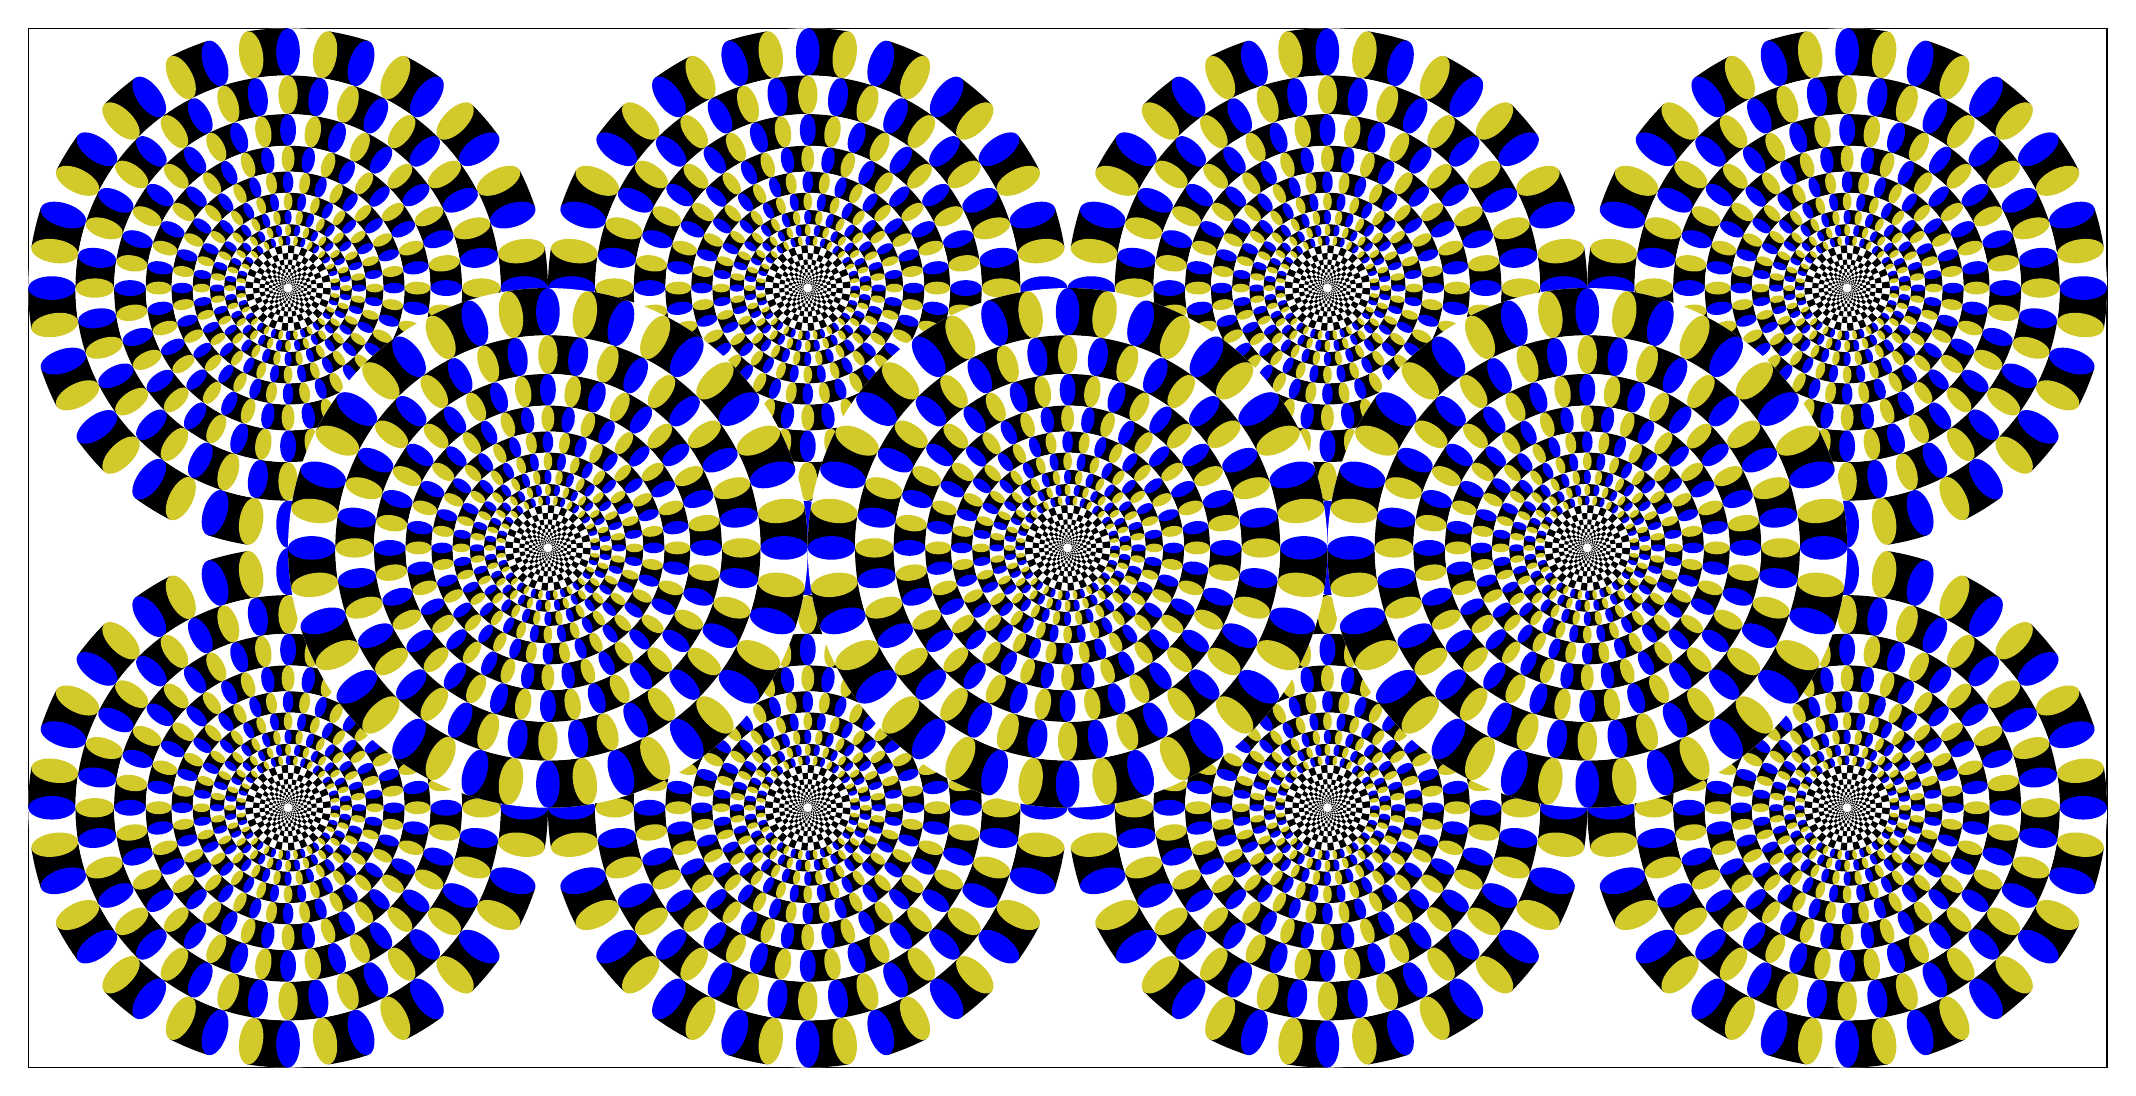
\begin{tikzpicture}
		\draw (-3.3,-3.3) rectangle (23.1,9.9);
		\foreach\x/\y in{
			0/1,    1/1,     2/1,     3/1,
			0/0,    1/0,     2/0,     3/0,
			   .5/.5,  1.5/.5,  2.5/.5
		}{
			\begin{scope}
				\tikzset{shift={(\x*6.6,\y*6.6)}, xscale=(-1)^(\x+\y)}
				\pgflowlevelsynccm
				\foreach\j in{1,...,20}{
					\draw[line width=6mm, white]
						circle[radius=3cm];
					\draw[line width=6mm, dash phase = \j*13.408pt,
						dash pattern = on 13.408pt off 13.408pt]
						circle[radius=3cm];
					\ifnum \j < 10
					\foreach\i in{1,...,20}{
						\tikzset{rotate=\i*18+\j*9}
						\fill [yellow!80!black]
							(3,0) ellipse[x radius=3mm, y radius=1.5mm];
						\tikzset{rotate=9}
						\fill [blue]
							(3,0) ellipse[x radius=3mm, y radius=1.5mm];
					}
					\fi
					\tikzset{scale=.81818}
					\pgflowlevelsynccm
				}
			\end{scope}
		}
	\end{tikzpicture}
\end{document}
